\chapter{Discussion}
In this chapter the work done in conjunction to this thesis will be discussed. 
First I will talk about the pros and cons using \gls{IBC} in \gls{NDN}.
Then I will discuss the \gls{HSS} and possible drawbacks in the system. 
Scalability issues and other applicable networks for the application will be mentioned.

\section{Named Data Networking}
\gls{NDN} facilitates a lot of concepts that shows to be a huge benefit for todays Internet, and the predicted increase of \gls{IoT}.
The naming of content and content routing provides usability to \gls{IoT}, and \gls{wsn}.
Bandwidth redundancy in the network is reduced, security properties in network layer is provided, and the linkage between data and its publisher is easily proven. 
It is easier for machines to directly communicate, without having to connect to a router.
Broadcast and multicast comes naturally, hence wireless communication can be done in a simple matter.

Network layer becomes ``smart''. 

Usability

Once a basic perception of the \gls{NDN} architecture is understood, it is easy to begin developing applications on top of \gls{NDN}.
The \gls{PyNDN2} framework comes with good examples of how to develop simple applications with packets that are signed and encrypted.

The concept of naming \gls{data} introduces more simplicity, but also a new way of application design thinking.
Addressing is dealt with one place in the architecture compared to an equivalent system over \gls{IP}. 
Security is easily applied in \gls{NDN}.


\section{Identity-Based Cryptography in Named Data Networking}
The concept of \gls{IBC} appears to be highly applicable to \gls{IoT} and \gls{wsn}~\cite{Patil:2012:SWS:2464778}, and so does \gls{NDN}. 
I believe that using \gls{IBC} in a \gls{wsn} combined with \gls{NDN} should make applications with security in this setting less complex and more practical than using RSA. 

Using \gls{ID} as public key eliminates the binding of ID and certificate. 
Compared to \gls{PKI} where the recipient have to download the public key certificate to verify the digital signature.
This is practical, less communication overhead to establish connection, lower energy consumption.
Less keys, IDs have to be known and distributed anyway (IP addresses).
DNS eliminated.
Exchanging data between nodes can be done completely without the \gls{PKG} after device registration.
However, there is issue of having a \gls{TTP}, i.e. the \gls{PKG}.
Generates all secret keys.
Single point of failure.
Only works for networks where users trust the \gls{PKG}. 
In \gls{wsn} this should not be a problem.
Typically networks that users might reacts to this kind of security structure could be telecommunication and email services. 
However, there is limited security in these types of network now anyway. 
Telcos have full control over all data flowing through their servers. 
Google states that their system is analyzing all content related to a Google user:
\begin{displayquote}
``Our automated systems analyse your content (including emails) to provide you personally relevant product features, such as customised search results, tailored advertising, and spam and malware detection. This analysis occurs as the content is sent, received, and when it is stored.''
~\cite{google_reads_email}
\end{displayquote}
The problem is that these actors do not want to make all content opaque for themselves, because they use it for their business. 
My point being, if this is going to be the case anyway in the future, when the network switches over to \gls{NDN} they could secure their systems with cryptography such as \gls{IBC} to make it more difficult for adversaries to eavesdrop or perform any other form of attacks.

Running this over \gls{NDN}, makes it even more practical, because of the naming of content concept that \gls{NDN} is built upon. 
Easier to secure data, relate data to publisher, and authenticate that the publisher is aware of what content it publish. 

Key revocation can be a problem.
In \gls{PKI} a device can create its own new key pair when compromised. 
This is not possible with \gls{IBC}.
One suggestion has been to add a monthly timestamp to the \gls{name}, but the the \gls{PKG} has to renew private keys for everybody each month. 
This solution do not scale very well due to a lot of computation at the \gls{PKG}.
With the \gls{FSM}, every user will be notified when a identity is revoked.
There is no use for periodically checking names.
But the renewal of keys might not be an issue in the \gls{HSS}. \todo{more..}

If the \gls{PKG} must renew its key pair, \gls{MSK} and \gls{MPK}.
Secret key renewal for all devices.

\todo{refactor this section}
Can authenticate \gls{data} even using insecure DNS or HTTP. 
There is only one linkage between the \gls{name} and the content, and if the user obtains the right \gls{MPK}, there is no doubt where the \gls{data} originates from and that it is not altered.
In RSA public key cryptography we have to find the key related to the signature. 
In worst case this will be equivalent of retrieving the \gls{MPK} each time, which is not likely. 
Or the \gls{MPK} can be appended to the message.

usability 

A comparison of \gls{pkc} and \gls{IBC} is shown in~\autoref{fig:ibc-pkc-comparison}.
\begin{figure}[ht]
  \centering
  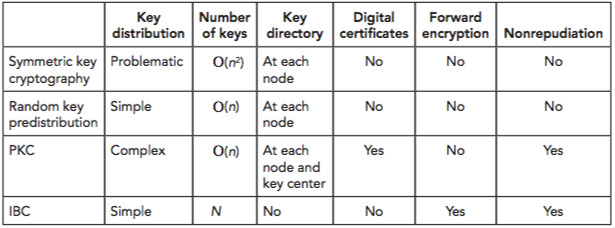
\includegraphics[width=1\textwidth]{ibc-comparison-in-wsn.png}
  \caption{Comparison with PKC and IBC ~\cite[Table 9.6]{Patil:2012:SWS:2464778}}
  \label{fig:ibc-pkc-comparison}
\end{figure}

\section{Health Sensor System}
The application is not tested on with real sensors, hence I cannot conclude with anything regarding the computational power of such devices, nor the life time of the battery when performing \gls{IBE}.  

Power efficiency
\todo{more on this}

A problem with \gls{wsn} in \gls{IP} networks, is that it is a limited number of \gls{IP} adderesses (especially in \gls{IPv4}).
So the global scalability issue arises due to the potentially large number of sensors that could be deployed. 
With the naming rules in \gls{NDN}, this is not a issue.

In~\autoref{ibc-performance} we can see that \gls{IBC} is performing better than regular asymmetric cryptography, RSA. 

Encrypting with same symmetric key for each set of \gls{data}, limits the encryption computation for the device if several devices requests the same \gls{data}.
Using a unique key for each time \gls{data} is requested is more secure and can be used for more sensitive content.

Who can play the role of a device?
As mentioned in~\autoref{rendezvous_authentication} and~\autoref{init} there should be a limitation of which devices that can be initialized to the trust domain.
\todo{hm... something here?}

Storing the \gls{SK} in a secure fashion.

Preloading secret key, offline mode, yet the initialization protocol should be used to do this, unless the sharing is done in a wired environment. 
\gls{NFC} signal is hard (impossible?) to eavesdrop, thus the initialization protocol is not needed. 


\section{Scalability}
Distributing the \gls{ID}-list can be an issue, as the list can grow linearly with the number of participants in the trust domain.
However, this might not be a huge problem in the use cases that is addressed in this thesis, considering that the number of devices in the \gls{HSS} will not grow larger than e.g. 100 devices. 

Example:
ID size * devices = x bytes 

\section{Sync}
The sync application makes it possible for users to know who has a valid public key within the \gls{PKG}s domain.
One drawback with the key distribution using \gls{FSM} is that for the sender to be 100\% sure that the message is encrypted with the latest \gls{ID}, the sender has to rely on that it has received the latest sync state available from the \gls{PKG}.
Likewise when a \gls{receiver} verifies a signature, it has to rely on the same principle to be able to know if the belonging \gls{ID} is still valid.
Since the scalability is not that big of an issue in this scenario, the monthly (or even more often) timestamp appended to the \gls{ID} might be a good solution to reduce the time of exposure when compromised.

There are some issues that could occur in such a system. 
\gls{DoS} on Sync \gls{interest} and Sync \gls{data}. 
If the \gls{FSM} is used to revoke public keys as suggested, an attacker who has found the compromised \gls{SK}, can try to deny the distribution of the new list, i.e. the Sync \gls{data}, from the distributor. 
This is however a complicated attack and an updated list would spread fast.
Performing \gls{DoS} on every node is not easy, and would block the network access for the adversary anyway.
In~\cite{DBLP:conf/spw/StajanoA99} Frank Stajano and Ross Anderson mentions possible \gls{DoS} attacks, such as radio jamming and battery exhaustion. 
All applications that relies on some sort of crucial information derived using \gls{FSM} (\autoref{file-sync}) are vulnerable to this kind of \gls{DoS}.

\section{Test Results}
IBE vs RSA

RTT on protocols



\section{Other Use Cases}
The trust model used in the \gls{HSS} can be used in any network where the use of a \gls{TTP} is accepted. 
Such a system can for instance be:
\begin{enumerate}
	\item Home automation systems
	\item \gls{BAS}
	\item \gls{BMS}
	\item Health care
	\item Military networks
	\item Sensor networks such as disaster, habitat and hazard monitoring
\end{enumerate}


